\documentclass[12pt]{optlab-bachelor} 
\usepackage{amsfonts}
\usepackage{amsmath,amssymb}
\usepackage{algorithm}
\usepackage{algorithmic}
\usepackage[dvipdfmx]{graphicx}

\def\年度{2017}
\def\氏名{天本 祐希}
\def\学生番号{15713004}
\def\題目{並列機械モデルにおける\\最大実行開始待ち時間最小化問題の計算論的分析}
\def\背題目{並列機械モデルにおける最大実行開始待ち時間最小化問題の計算論的分析}

\renewcommand{\bibname}{参考文献}

\begin{document}
\frontmatter

\chapter{はじめに}
\section{研究背景}
一般に,Webアプリケーションサービスを運用している会社では,運用しているWebアプ
リケーションの応答が遅いと,顧客離れやクレームの被害を受けることがある.
そのため,計算サーバーの応答の早さは重要である.応答の早い計算サーバー
を作るためには,与えられたタスクをどのように割り当て,処理するかを考える必要がある.
計算サーバーのタスクの処理開始は,Webサービスの利用者が,ネットワーク
を介して,そのサービスを運用している会社の計算サーバーにタスクの処理の
要求を行い,そのタスクが計算サーバーに到着した後である.そのため,タス
クの到着時刻とは,タスク処理の処理開始可能時刻である.最大実行開始待ち時間
最小化問題とは,処理開始可能時刻を制約とし,タスクが到着してから,タス
ク処理が開始されるまでの時間,つまり,Webサービス利用者の不満の最小化
を目的とするスケジューリング問題である.また,割り当てるタスクの情報が
あらかじめわからない点から,計算サーバーへのはタスク割り当てはオンライ
ン環境で行われると言える.したがって,計算サーバーへのタスク割り当ては,
最大実行開始待ち時間最小化を目的とするオンラインスケジューリング問題と
して捉えることができる.スケジューリング問題では,タスクをジョブと表記する.
この問題は,ジョブを処理する機械数がいずれの場合においても,問題の難し
さは明らかになっていない.

実行開始待ち時間を軸にとって従来研究を調査したところ,実行開始待ち時
間を目的関数とする問題の多くは未だ研究されていないことが明らかとなった.

\section{研究目的}
最大実行開始待ち時間最小化問題はどの機械モデルにおいても計算複雑さが
明らかでなく,問題の難しさに与える影響の本質は現れていない.
また,制約が問題に与える影響も明らかではない.
本研究の目的は,問題を定式化し,扱う問題の計算複雑さを明らかにすることと,解放の提案である.また,
機械モデルが問題の計算複雑さに与える影響についても扱う.

\section{研究成果}
本研究では,最大実行開始待ち時間最小化問題を決定問題として捉えたとき,
無関連並列機械モデルにおいて,NP完全であることを明らかにした.

\section{章構成}
第2章では,最大実行開始待ち時間最小化問題の定式化を行なう.また,NP
完全性の証明の際に用いる,最大実行開始待ち時間最小化問題を決定問題と
して捉えたときの定式化も行なう.

第3章では,本研究で扱う問題に関連する,JITジョブ荷重和最大化問題と
処理開始可能時刻付き最大遅れ時間最小化問題に対する従来研究の成果を,計
算複雑さの観点,解法の開発に用いられる手法の観点から,それぞれまとめる.

第4章から第5章にかけて,本研究の成果を述べる.第4章では,まず,無
関連並列機械モデルにおける最大実行開始待ち時間最小化問題の計算複雑さに
ついて述べる.

第5章では,・・・

第7章では,結論として,本研究の成果と今後の課題を述べる.

\chapter{問題の定式化}
\section{最大実行開始待ち時間最小化問題}
最大実行開始待ち時間最小化問題とは,各ジョブの処理開始可能時刻を制約
とし,処理開始可能時刻と処理開始時刻の差の最大値の最小化を目的とするス
ケジューリング問題である.以下の前提のもと,
\begin{itemize}
\item 各機械は,あるジョブの処理の完了と同時に異なるジョブの処理を開始
  できるが,複数のジョブを同時に処理するkとはできない
\item 各ジョブの処理は任意の1機械の処理で完了する
\item 各ジョブの処理を開始すると,完了するまで中断しない
\end{itemize}
処理開始可能時刻の制約を満たすスケジュールのうち,最大実行開始待ち時間
を最小とするスケジュールを求める.

各ジョブを処理する機械の性能によって,機械モデルは次のように分類され
る.まず,ジョブを処理する機械の台数について,一つの機械で処理する単一
機械モデルと,複数の機械で処理を行なう並列機械モデルに分類される.並列
機械モデルはさらに,全ての機械の性能が等しい同一並列機械モデル,機械ご
とに処理速度が異なる一様並列機械モデル,ジョブと機械の組み合わせによっ
て処理時間が異なる無関連並列機械モデルに分類される.

以下では,無関連並列機械モデルについて,最大実行開始待ち時間最小化問
題を定式化する.\\

\noindent \textbf{入力:}

ジョブの集合 $\mathcal{J}$ を無関連機械の集合 $\mathcal{M}$と表記し,
$J \in \mathcal{J}$ を $M \in \mathcal{M}$ で処理する.
処理開始可能時刻関数 $r : \mathcal{J} \to \mathbb{N}$,処理
時間関数 $p : \mathcal{J} \times \mathcal{M} \to \mathbb{N}$
であり,それぞれの関数が返す値は自然数である.入力は2項組,$(p,r)$ と
表す.\\

\noindent \textbf{解:}

問題の前提に基づき,スケジュールを定式化する.スケジュールは以下の条
件を満たす $A : \mathcal{J} \to \mathcal{M}$ と $S : \mathcal{J} \to
\mathbb{N}$ の対$(A,S)$ であり,スケジュールによって,各ジョブを,どの
機械で,いつ処理するかを決める.
\begin{itemize}
\item $\forall J \in \mathcal{J}\big[s(J) \ge r(J) \big]$
  \begin{itemize}
  \item 各ジョブは処理開始可能時刻以降に処理を開始する
  \end{itemize}
\item $\forall J, J' \in \mathcal{J}\ \Big[ \big[J\neq J' \land A(J) = A(J')\big] \Rightarrow [s(J), s(J)+p(J,A(J))) \cap[s(J'), s(J')+p(J', A(J'))) = \emptyset \Big]$
  \begin{itemize}
  \item 各機械は同時に複数のジョブを処理しない
  \item 各ジョブの処理を開始すると,完了するまで中断しない
  \end{itemize}
\end{itemize}

\noindent \textbf{目的関数:}

実行可能なスケジュール $(A,S)$ のうち,最大の実行開始待ち時間,
$$\varphi(A,S) = \displaystyle \max_{J \in \mathcal{J}}\{s(J) -
r(J)\}$$
を最小とするスケジュールを求める.

\section{最大実行開始待ち時間最小化問題(決定問題)}
最大実行開始待ち時間最小化問題(決定問題)とは,各ジョブの処理開始可能時刻を制約
とし,処理開始可能時刻と処理開始時刻の差の最大値が $w$ 以下となるスケ
ジュールが存在するかを判定する問題である.以下の前提のもと,
\begin{itemize}
\item 各機械は,あるジョブの処理の完了と同時に異なるジョブの処理を開始
  できるが,複数のジョブを同時に処理するkとはできない
\item 各ジョブの処理は任意の1機械の処理で完了する
\item 各ジョブの処理を開始すると,完了するまで中断しない
\end{itemize}
処理開始可能時刻の制約を満たすスケジュールのうち,最大実行開始待ち時間
が $w$ 以下となるスケジュールが存在するかを判定する.

各ジョブを処理する機械の性能によって,機械モデルは次のように分類され
る.まず,ジョブを処理する機械の台数について,一つの機械で処理する単一
機械モデルと,複数の機械で処理を行なう並列機械モデルに分類される.並列
機械モデルはさらに,全ての機械の性能が等しい同一並列機械モデル,機械ご
とに処理速度が異なる一様並列機械モデル,ジョブと機械の組み合わせによっ
て処理時間が異なる無関連並列機械モデルに分類される.

以下では,無関連並列機械モデルについて,最大実行開始待ち時間最小化問
題を定式化する.\\

\noindent \textbf{Instance:}

ジョブの集合 $\mathcal{J}$ を無関連機械の集合 $\mathcal{M}$と表記し,
$J \in \mathcal{J}$ を $M \in \mathcal{M}$ で処理する.
処理開始可能時刻関数 $r : \mathcal{J} \to \mathbb{N}$,処理
時間関数 $p : \mathcal{J} \times \mathcal{M} \to \mathbb{N}$,実行開始
待ち時間 $w$ であり,それぞれの関数が返す値は自然数である.入力は3項組,$(p,r,w)$ と
表す.\\

\noindent \textbf{Question:}

以下の条件を満たす $A : \mathcal{J} \to \mathcal{M}$ と $S : \mathcal{J} \to
\mathbb{N}$ の対$(A,S)$ が存在するかどうか.
\begin{itemize}
\item $\forall J \in \mathcal{J}\big[s(J) \ge r(J) \big]$
  \begin{itemize}
  \item 各ジョブは処理開始可能時刻以降に処理を開始する
  \end{itemize}
\item $\forall J, J' \in \mathcal{J}\ \Big[ \big[J\ne J' \land A(J) = A(J')\big] \Rightarrow [s(J), s(J)+p(J,A(J))) \cap[s(J'), s(J')+p(J', A(J'))) = \emptyset \Big]$
  \begin{itemize}
  \item 各機械は同時に複数のジョブを処理しない
  \item 各ジョブの処理を開始すると,完了するまで中断しない
  \end{itemize}
\item $\max\big\{s(J) - r(J) \mid J \in \mathcal{J}\big\} \le w$
  \begin{itemize}
  \item ジョブの処理開始可能時刻からその処理を開始するまでの待ち時間は $w$ 以下
  \end{itemize}
\end{itemize}

また,実行開始待ち時間 $w$ の制約が最も強い場合,つまり,$w = 0$ の
とき,各ジョブは処理開始可能時刻ちょうどで処理を開始しなければならない
ので,JITジョブスケジューリング問題に対応する.
また,処理開始可能時刻 + 処理時間 + 実行開始待ち時間 = 納期 と考えるこ
とで,処理開始可能時刻と納期付きのスケジューリング問題として対応づけることができる.
以上より,最大実行開始待ち時間最小化問題の従来研究として,JIT ジョブ荷
重和最大化問題と最大遅れ時間最小化問題について,成果を紹介する.


\chapter{従来研究}
ここでは,JITジョブ荷重和最大化問題と,処理開始可能時刻付き最大遅れ
時間最小化問題について,従来研究の成果と,解法の開発手法を紹介する.

\section{JITジョブ荷重和最大化問題} %参考文献:川俣さんの論文
この問題は 3-SAT からの還元により,強 NP 困難であることが証明されて
いる().JIT ジョブ荷重和最大化問題と 3-SAT の定義は以下である.\\

\noindent \textbf{入力:}

$n$ 個のジョブ $J_1,\ldots,J_n$ を $m$ 台の同一機械 $M_1,\ldots,M_m$
で処理する.入力は,各ジョブ $J_i ( i \in \{1,\ldots,n\} )$ の,処理時
間 $p_i$ ,処理開始可能時刻 $r_i$ ,納期 $d_i$ ,荷重 $w_i$ であり,
それぞれの値は自然数である.
各ジョブの処理時間をまとめて $P = (p_1,\ldots,p_n) \in \mathbb{N}^n$,
処理開始可能時刻をまとめて $R = (r_1,\ldots,r_n) \in \mathbb{N}^n$ ,
納期をまとめて $D = (d_1,\ldots,d_n) \in \mathbb{N}^n$ ,
荷重をまとめて $W = (w_1,\ldots,w_n) \in \mathbb{N}^n$ と表し,
入力 は 4 項組,$(P,R,D,W)$ と表す.\\

\noindent \textbf{解:}

問題の前提に基づき,スケジュールを定式化する.スケジュールは以下
の条件を満たす $\forall j \in \{1,\ldots,m\}\big[A_j \subseteq
\{1,\ldots,n\}\big]$ と $C : \{1,\ldots,n\} \to \mathbb{N}$ の対 $(A,
C)$ であり,スケジュールによって,各ジョブを,どの機械で,いつ処理をするかを決める.
\begin{itemize}
\item $\forall i, i' \in \{1,\ldots,n\}\ \Big[ \big[i \neq i' \land A_i =
  A_{i'}\big] \Rightarrow [C(i) - p_j, C(i)) \cap [C(i') - p_{i'}, C(i')) = \emptyset \Big]$
\item  $\forall i \in \{1,\ldots,n\}\big[C(i) - p_i \ge r_i\big]$
\end{itemize}

\noindent \textbf{目的関数:}

実行可能なスケジュール $(A, C)$ のうち,納期以前に処理を完了するジョ
ブの荷重和,
$$\displaystyle \varphi(A,C) = \sum_{i \in \mathcal{Q}(A,C)}w_i$$,
$i \in \mathcal{Q}(A,C)$ を最大とするスケジュールを求める.ただし,
$\mathcal{Q}(A, C)$ はスケジュール $(A, C)$ に
おいて納期以前に処理を完了するジョブの集合である (
$\mathcal{Q}(A, C) = \{i \in \{1,\ldots, n\} | C(i) \ge d_i \}$ ).\\

\noindent \textbf{Instance:}

ブール型の変数集合 $X$ と,$X$ 上の 3 つのリテラル
からなる集合の集合 $H$ (各 $h \in H$ は $|h| = 3$ を満たす).

\noindent \textbf{Question:}

$H$ を充足する真理値割り当て $f ; X \to \{0,1\}$,
つまり,
$$\displaystyle \bigwedge_{h \in H} \bigg(\bigvee_{x \in h}f(x) \lor
\bigvee_{\bar x \in h}\lnot f(x) \bigg) = 1$$
を満たす $f$ が存在するか?\\

ブール型変数の集合 $X = \{x_1,\ldots,,x_β\}$ と, $X$ 上の 3 つのリテラル
からなる集合 $H = {h_1,\ldots,h_{\lambda}}$ の 2 項組, $(X,H)$ を任意の
3-SAT 問題の入力とする.
議論に先立ち,いくつかの表記を導入する.各 $k \in \{1,\ldots,\beta\}$
について, $\gamma_k$ を $H$ に おいて $x_k$ が現れる回数を表す自然
数とし, $\gamma$ を $\gamma_k ( k \in \{1,\ldots,\beta\} )$の最大値に
1 を加えた値とする($\displaystyle \gamma = \max_{k \in \{1,2,\ldots, \beta\}} \{\gamma_k \}+ 1$).
$(X, H)$ に基づき,以下のように JIT ジョブ荷重和最大化問題の入力
を設定する. $2\beta_{\gamma}$ 個のジョブを $\lambda + \beta$ 台の
無関連機械で処理する.各ジョブの処理時間,納期ズレ幅,納期,荷
重を以下のように設定する.\\

\noindent \textbf{納期ズレ幅の設定}

各ジョブ $i \in \{1,\ldots,2\beta \gamma\}$ の納期ズレ幅
$\alpha_i$ を 0 とする.\\

\noindent \textbf{納期の設定}

$\{1,2,\ldots, \beta \gamma\}$$ の $$\beta \gamma$ 個ジョブの納期につ
いて,昇順で $\gamma$ 個ずつとった $\beta$ 個のグループについて,機械
を順に対応させる.
各グループ $k \in \{1,2,\ldots, \beta\}$ の $\gamma$ 番目のジョブの納
期を $2\gamma - 1$,$\ell$ 番目のジョブ ( $\ell \neq \gamma$ ) の納期
を $\ell$ とする.つまり,各 $k \in \{1,2,\ldots, \beta\}$ と $\ell \in \{1,2,\ldots,
\gamma\}$について,
$$d_{(k - 1)\gamma + \ell} = \left\{ \begin{array}{ll} \ell & \text{if } \ell < \gamma \\ 2\gamma - 1 & \text{if } \ell = \gamma \end{array} \right.$$
$\{\beta \gamma + 1,\ldots, 2\beta \gamma\}$ の $\beta \gamma$ 個のジョ
ブの納期についても,同様に対応させる.
各グループ $k \in \{1,2,\ldots, \beta\}$ の $\gamma$ 番目のジョブの納期を $\gamma$,$\ell$ 番目のジョブ ( $\ell \neq \gamma$ ) の納期を $\gamma + \ell$ とする.
つまり,各 $k \in \{1,2,\ldots, \beta\}$ と $\ell \in \{1,2,\ldots,
\gamma\}$について,
$$d_{(\beta + k - 1)\gamma + \ell} = \left\{ \begin{array}{ll}\gamma +  \ell & \text{if } \ell < \gamma \\ \gamma & \text{if } \ell = \gamma \end{array} \right.$$

\noindent \textbf{荷重和の設定}

各ジョブを納期昇順に基づき $2\beta$ 個のグループに分ける.
グループ $k \in \{1,2,\ldots,\beta\}$ と,グループ $k + \beta$ について,グループの $\gamma$ 番目のジョブの荷重を $\gamma$ とし,それ以外のジョブの荷重を 1 とする.
つまり,各 $k \in \{1,2,\ldots, \beta\}$ と $\ell \in \{1,2,\ldots,
\gamma\}$について,
$$w_{(k - 1)\gamma + \ell^v} = w_{(\beta + k - 1)\gamma + \ell} = \left\{ \begin{array}{ll} 1 & \text{if } \ell < \gamma \\ \gamma & \text{if } \ell = \gamma \end{array} \right.$$

\noindent \textbf{処理時間の設定}

各ジョブを納期昇順に基づき $2\beta$ 個のグループに分ける
グループ $k \in \{1,2,\ldots,\beta\}$ に機械を $k$ に対応させ,グルー
プ $k + \beta$ にも同様に機械 $k$ を対応させる.各グループの各ジョブについて, グループに対応した機械以外の各機械における処理時間を $2\gamma$ とする.
各グループの $\gamma$ 番目のジョブの,グループに対応する機械における処
理時間を $\gamma$ とし,$\gamma$ 番目のジョブをのぞいた各ジョブの,グループに対応する機械における処理時間を 1 とする.
つまり,各 $j \in \{1,2,\ldots, \beta\}$ と $k \in \{1,2,\ldots,
\beta\}$ と $\ell \in \{1,2,\ldots, \gamma\}$について,
$$p_{(k - 1)\gamma + \ell, j} = p_{(\beta + k - 1)\gamma + \ell, j} = \left\{ \begin{array}{ll} 1 & \text{if } \ell < \gamma \text{ and } j = k, \\ \gamma & \text{if } \ell = \gamma \text{ and } j = k, \\ 2\gamma & \text{otherwise}\end{array} \right.$$

残りの各機械 $j \in \{\beta + 1, \ldots , \beta + \gamma\}$ について,各ジョブの処理時間を設定する
各グループ $k \in \{1,2,\ldots,\beta\}$ について,$x_k$ を対応させる.
各グループ $k \in \{1,2,\ldots,\beta\}$ について,$\ell \in \{1,2,\ldots, \gamma - 1\}$ 番目の各ジョブにつ いて,$x_k \in h_{j - \beta}$ であれば $d_{(k - 1)\gamma + 1}$ とし,そうでない場合は $2\gamma$ とする.また,$\gamma$ 番目 のジョブの処理時間は $2\gamma$ とする.
グループ $k + \beta$ について$\bar x_k$ を対応させる.
$\ell \in \{1,2,\ldots, \gamma - 1\}$ 番目の各ジョブについて,$\bar x_k \in h_{j - \beta}$ であれば $d_{(\beta + k - 1)\gamma + \ell}$ とし, そうでない場合は $2\gamma$ とする.また,$\gamma$ 番目のジョブの処理時間は $2\gamma$ とする.
つまり,各 $j \in \{\beta + 1,\ldots, \beta + \gamma\}$ と $k \in
\{1,2,\ldots, \beta\}$ と $\ell \in \{1,2,\ldots, \gamma\}$について,
$$p_{(k - 1)\gamma + \ell, j} = \left\{ \begin{array}{ll} d_{(k - 1)\gamma + 1} & \text{if } \ell < \gamma \text{ and } x_k \in h_{j - \beta}, \\ 2\gamma & \text{otherwise} \end{array} \right.$$

$$p_{(\beta + k - 1)\gamma + \ell, j} = \left\{ \begin{array}{ll} d_{(\beta + k - 1)\gamma + \ell} & \text{if } \ell < \gamma \text{ and } \bar x_k \in h_{j - \beta}, \\ 2\gamma & \text{otherwise} \end{array} \right.$$

このように設定した $(P,a,D,W)$ は JIT ジョブ荷重和最大化問題の入力である.以降,$(X,H)$ に基づいて前述のように設定した $(P,a,D,W)$ を区別して $I_{(X,H)}$ と表す $(I_{(X,H)} = (P,a,D,W))$.
以下,$H$ を充足する真理値割り当て $f : X \to \{0,1\}$ が存在すること
と,$I_{(X,H)}$ を入力とする JIT ジョブ荷重和最大化問題に対して
$\varphi(A,C) \ge \beta(2\gamma - 1) + \lambda$ を満たす実行可能なスケ
ジュール $(A,C)$ が存在することが,同値であることを示す.\\

\noindent \textbf{補題 1}
$H$ を充足する真理値割り当て $f : X \to \{0,1\}$ が存在するならば,
$I_{(X,H)}$ を入力とする JIT ジョブ荷重和最大化問題に対して
$\varphi(A, C) \ge \beta(2\gamma - 1) + \lambda$ を満たす実行可能なス
ケジュール $(A, C)$ が存在する.\\ 

\begin{proof}
  $(X,H)$ を任意の 3 -SAT 問題の入力とし, $f : X \to \{0,1\}$ を $H$ を
  充足する真理値割り当てとする.つまり, $f$ は以下を満たす.
  $$\displaystyle \bigwedge_{h \in H} \bigg(\bigvee_{x \in h}f(x) \lor
    \bigvee_{\bar x \in h}\lnot f(x) \bigg) = 1$$
  各 $k \in \{1,\ldots, \beta\}$ について, $f(x_k) = 1$ ならばグルー
  プ $\beta + k$ の全てのジョブを,グループ $\beta + k$ に対応する機械
  $k$ に割り当て,そうでなければグルー
  プ $k$ の全てのジョ ブを,グループ $k$ に対応する機械 $k$ に割り当てる.ま
  た,機械 $k$ に割り当てた各ジョ ブの完了時刻を納期とする.つまり,
  $f(x_k) = 1$ ならば,各 $\ell \in \{1,\ldots,\gamma\}$ について $A_k
  :=A_k cup\{(\beta+k−1)\gamma+\ell\}$ かつ
  $C((\beta+k−1)\gamma+\ell)=d(\beta+k−1)\gamma+l$ ,$f(x_k)=0$ なら
  ば,各 $\ell \in \{1,\ldots,\gamma \}$ について$A_k :=A_k \cup
  \{(k−1)\gamma+\ell \}$ かつ $C((k−1)\gamma+\ell)=d(k−1)\gamma+\ell$
  . $I_{(X,H)}$ の定義より,ここまでのスケジュールにおいて,機械
  $1,\ldots, \beta$ に割り当てたジョ ブの処理時間は重複せず (図 A.1),完
  了時刻は納期であることから,$k \in \{1,\ldots,\beta\}$ に割り当てたジョ
  ブは JIT ジョブである.よって,ここまでのスケジュール $(A, C)$ における
  JIT ジョブの荷重和は,
  $$\displaystyle \varphi(A,C) = \sum_{k \in
    \{1,\ldots,\beta\}}\bigg(\sum_{i \in \mathcal{Q}(A,C):i \in
    A_k}w_i\bigg) = \sum_{k \in \{1,\ldots,\beta\}}(2\gamma - 1) =
  \beta(2\gamma - 1)$$.
  \begin{center}
    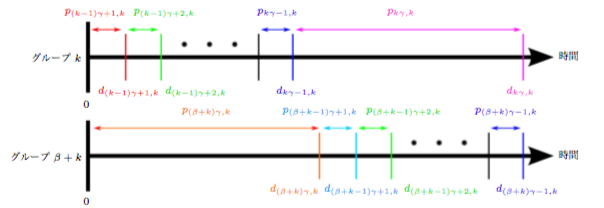
\includegraphics[width = 15cm]{SJIT1.png} \\
    図 $A.1$ : 機械 $k \in \{1,\ldots,\beta\}$ に対応するグループ $k$
    とグループ $\beta + k$ の各ジョブ
  \end{center}
  各 $j\in \{1,\ldots,\lambda\}$ について,$f(x_k)=1$ を満たす$x_k \in
  h_j$ か,$f(x_k)=0$ を満たす $\bar x_k \in h_j$ をひとつ見つける. $f$ が $H$ を充足することから,各 $j \in \{1,\ldots,\lambda\}$ について, 上記を満たすリテラルは必ず存在する.
  与えられた $j \in \{1,\ldots,\lambda \}$ について, $f(x_k) = 1$ を満
  たす $x_k \in h_j$ を見つけたと仮定す る.グループ $k$ のジョブ
  のうち,いずれの機械にも割り当てられていない $\ell \in
  \{1,\ldots,\gamma - 1\}$ を見つける.グループ $k$ のジョブは,
  $f (x_k) = 1$ であることから,$\{1,\ldots, \beta \}$ のいずれの機
  械にも割り当てられておらず,また,各リテラルが現れる回数は高々
  $\gamma − 1$ であることから,そのような $\ell$ 番目のジョブは必す
  ゙存在する. $A_{j + \beta} := A_{j + \beta} \cup \{ (k − 1) \gamma +
  \ell\}$ とし, $C((k − 1)\gamma + l) = d(k−1)\gamma + \ell$ とする.
  次に,与えられた $j \in \{1,\ldots,\lambda\}$ について, $f(x_k) = 0$
  を満たす $\bar x_k \in h_j$ を見つけたと仮定する.グループ $\beta
  + k$ のジョブのうち,いずれの機械にも割り当てられていない $\ell
  \in \{1,\ldots,\gamma\}$ を見つける.先ほどと同様の議論で,そのよ
  うな $\ell$ は必ず存在する. $A_{j + \beta} := A_{j + \beta} \cup \{
  (\beta + k − 1 ) \gamma + \ell \} = j + \beta$ とし,$C((\beta + k −
  1) \gamma + \ell) = d(\beta + k − 1)\gamma + \ell$ とする.
  各グループの $\ell \in \{1,\ldots,\gamma − 1\}$ 番目のジョブ
  の荷重が 1 であることから,各 $j \in \{1,\ldots, \lambda \}$ につ
  いて $j$ に割り当てられた JIT ジョブの荷重和は,
  $$\displaystyle \sum_{i \in \mathcal{Q}(A,C):A(i) = j + \beta}w_i =
  1$$
  ここまでのスケジュール $(A, C)$ においていずれの機械にも割り当てられて
  いないジョブを, $\max\{d_i | i \in \{1,\ldots, 2\beta \gamma\}$ のあと,任意の順,任意の機械で処理するものとする.
  明らかにスケジュール $(A, C)$ は実行可能であり,以下を満たす.
  $$\displaystyle \varphi(A,C) = \sum_{j \in
      \{1,\ldots,\beta\}} \sum_{i \in \mathcal{Q}(A,C):i \in
      A_j}w_i + \sum_{j \in
      \{\beta + 1,\ldots,\lambda + \beta\}} \sum_{i \in \mathcal{Q}(A,C):i \in
      A_j}w_i =
    \beta(2\gamma - 1) + \lambda$$.
\end{proof}

ここで, $I_{(X,H)}$ を入力とする JIT ジョブ荷重和最大化問題に
おける実行可能なスケジュールについて,いくつかの性質を示す.
$(A, C)$ を $_{I(X,H)}$ を入力とする JIT ジョブ荷重和最大化問題に
おける任意の実行可能なスケジュールとする.実行可能性の制約により,各シ
゙ョブは機械の稼働開始時刻以降に処理を開始することから,各 JIT ジョ
ブ $i \in \mathcal{Q}(A,C)$ について,$C(i) − p_i = d_i − p_i \ge 0$ であ
る.このことから,$p_i,j \ge 2\gamma$ かつ $d_i \le 2\gamma − 1$ を満
たす $i \in \{1,\ldots,n\}$ と $j \in \{1,\ldots,m\}$ について,$i \in
\mathcal{Q}(A,C)$ のとき,$i \notin A_j$ である.したがって,
$I_{(X,H)}$ の定義より,各 $k \in \{1,\ldots,\beta\}$ について,
\begin{itemize}
\item $i \in \mathcal{Q}(A,C)$ かつ $i \in A_k$ ならば,
  $(k − 1)\gamma + 1 \le i \le k\gamma$ または $(\beta + k − 1)\gamma +
  1 \le i \le (\beta + k)\gamma$ である.
\item $k\gamma \in \mathcal{Q}(A,C)$ ならば $k\gamma \in A_k$ であ
  り,$\beta + k)\gamma \in \mathcal{Q}(A,C)$ な
  らば $(\beta + k)\gamma \in A_k$ である.
\end{itemize}
実行可能性の制約より,同じ機械に割り当てられた複数のジョブの処理
は重複しないこと から,各 $k \in \{1,\ldots,\beta\}$ について,
\begin{itemize}
\item $k\gamma \in \mathcal{Q}(A,C)$ ならば,$i \in A_k$ である任
  意の $i \in \mathcal{Q}(A,C)$ について,$i$ は $(k − 1)\gamma− 1
  \le k\gamma$ を満たす (図 $A.1$).
\item $(\beta + k)\gamma \in \mathcal{Q}(A,C)$ ならば,$i \in A_k$ て
  ゙ある任意の $i \in \mathcal{Q}(A,C)$ について,$i$ は
  $(\beta + k − 1)\gamma − 1 \le i \le (\beta + k)\gamma$ を満たす.
\end{itemize}
以上の議論より,各 $k \in \{1,\ldots, \beta \}$ について,$k$ に割り当
てられた JIT ジョブの荷重和は以下を満たし,
$$\sum_{i \in \mathcal{Q}(A,C):i \in A_k}w_i \le
2\gamma - 1 \label{A.1}$$

% タグづけがまだできていない
以下のいずれかを満たす場合にのみ,$\displaystyle \sum_{i \in \mathcal{Q}(A,C):i \in A_k}w_i =
2\gamma - 1$ となる.
\begin{itemize}
\item $\{i \in \mathcal{Q}(A,C) \mid i \in A_k\} = \{(k - 1)\gamma + 1, (k
  - 1)\gamma + 2,\ldots,k\gamma\} \label{A.2}$
\item $\{i \in \mathcal{Q}(A,C) \mid i \in A_k\} = \{(\beta + k -
  1)\gamma + 1, (\beta + k
  - 1)\gamma + 2,\ldots,(\beta + k)\gamma\} \label{A.3}$
\end{itemize} 
さらに,各 $j \in \{\beta + 1,\ldots, \beta + \lambda \}$ について,
各ジョブ $i \in \{1,\ldots, 2\beta \gamma \}$ の処理時間は $p_ij
\in \{d_i, 2\gamma \}$ であり,機械 $j$ に割り当てられるジョブは
高々 1 つである ( $|\{i \in \mathcal{Q}(A, C)\} | i \in A_j \}| \le 1$
).既に述べたように,各 $k \in \{1,\ldots,\beta \}$ について
$k\gamma \in \mathcal{Q}(A,C)$ ならば $k\gamma \in A_k$ であり,
$(\beta + k) \gamma \in \mathcal{Q}(A,C)$ ならば,$(\beta +
k)\gamma \in A_k$ である.これらのジョブをのぞいた各ジョブの荷
重は 1 であることから,各 $j \in \{ \beta + 1,\ldots,
\lambda + \beta \}$ について,
$$\displaystyle \sum_{i \in \mathcal{Q}:i \in A_j}w_i \le 1 \label{A.4}$$

\noindent \textbf{補題 2}
$I_{(X,H)}$ を入力とする JIT ジョブ荷重和最大化問題に対して
$\varphi(A, C) \ge \beta(2\gamma − 1) + \lambda$ を満たす実行可能なス
ケジュール $(A, C)$ が存在するならば,$H$ を充足する真理値割り当
て $f : X \to \{0, 1\}$ が存在する.

\begin{proof}
  $(A, C)$ を $I_{(X,H)}$ を入力とする JIT ジョブ荷重和最大化問題に
  対して $\varphi(A, C) \ge \beta (2\gamma − 1) + \lambda$ を満たす実行
  可能なスケジュールとする.式 ($15$) と式 ($A.4$) より $\varphi(A, C
  )\le≤ \beta(2\gamma − 1) + \lambda$ であり,このことから,
  $\varphi(A, C) = \beta (2\gamma − 1) + \lambda$ である.
  各機械 $k \in \{1,\ldots, \beta\}$ について,式 ($A.2$) または式
  ($A.3$) が満たされ,各 $j \in \{ \beta + 1,\ldots,\beta + \lambda
  \}$ について,$|\{ i \in \mathcal{Q}(A,C) | i \in A_j \} | = 1$ で
  ある.$(A,C)$ に基づき,$f : H \to \{0,1\}$ を以下のように設定する.
  各 $k \in \{1,\ldots, \beta \}$ について,式 ($A.3$) が満たされる
  ならば $f(x_k) = 1$ とし,そうでなければ $f(x_k) = 0$ とする.
  明らかに,各 $j \in \{\beta + 1,\ldots,\beta + \lambda \}$ について
  $j$ に割り当てられたただ一つの JIT ジョブ $i \in
  \mathcal{Q}(A,C)$ が存在し,$i \ge \beta \gamma$ ならば $f(x_k)
  = 1$ を満たすある $x_k \in h_{j - \beta}$ が存在し,$i > \beta
  \gamma$ ならば $f(x_k) = 0$ を満たすある $\bar x_k \in h_{j -
    \beta}$ が存在する.したがって,$f$ は $H$ を充足する真理値割り当てである.
\end{proof}

補題 1 と補題 2 より,$H$ を充足する真理値割り当て $f : X \to \{0,
1\}$ が存在することと,$I_{(X,H)}$ を入力とする JIT ジョブ荷重和
最大化問題に対して $\varphi(A, C) \ge \beta(2\gamma − 1) + \lambda$
を満たす実行可能なスケジュール $(A, C)$ が存在することは,同値で
ある.
3 -SAT 問題の入力 $(X,H)$ に基づく $I_{(X,H)}$ の生成に要する計算時
間は,明らかに多項式時間であり,入力 $I_{(X,H)}$ の長さは,$(X, H)$
の長さに関する多項式で表すことができる.したがって,無関連並列
機械モデルにおいて機械数が入力の一部の場合, JIT ジョブ荷重和
最大化問題は強 NP 困難である.

\section{処理開始可能時刻付き最大遅れ時間最小化問題} %生産管理1 Chapter3
この問題は 3-PARTITION からの還元により,強 NP 困難であることが証明さ
れている.処理開始可能時刻付き最大遅れ時間最小化問題と 3-PARTITION の
定義は以下である.\\

\noindent \textbf{入力:}

$n$ 個のジョブ $J_1,\ldots,J_n$ を 1 台の機械で処理する.入力は,各ジョ
ブ $J_i ( i \in \{1,\ldots,n\} )$ の,処理時間 $p_i$,処理開始可能時刻
$r_i$,納期 $d_i$ であり,それぞれの値は自然数である.各ジョブの処理時間をまとめて $P =
(p_1,\ldots,p_n) \in \mathbb{N}^n$ ,処理開始可能時刻をまとめて $R =
(r_1,\ldots,r_n) \in \mathbb{N}^n$ ,納期をまとめて $D =
(d_1,\ldots,d_n) \in \mathbb{N}^n$ と表し,入力は 3項組 $(P,R,D)$ と表
す.

\noindent \textbf{解:}

問題の前提に基づき,スケジュールを定式化する.スケジュールは以下
の条件を満たす $C : \{1,\ldots,n\} \to \mathbb{N}$ であり,スケジュー
ルによって,各ジョブ,をいつ処理をするかを決める.
\begin{itemize}
\item $\forall i, i' \in \{1,\ldots,n\}\ \Big[ \big[i \neq i' \big] \Rightarrow [C(i) - p_i, C(i)) \cap [C(i') - p_{i'}, C(i')) = \emptyset \Big]$
  \begin{itemize}
  \item 機械は同時に複数のジョブを処理しない
  \item 各ジョブの処理を開始すると,完了するまで中断しない
  \end{itemize}
\item  $\forall i \in \{1,\ldots,n\}\big[C(i) - p_i \ge r_i\big]$
  \begin{itemize}
  \item 各ジョブは処理開始可能時刻以降によりを開始する
  \end{itemize}
\end{itemize}

\noindent \textbf{目的関数:}

実行可能なスケジュール $C$ のうち,最大の納期遅れ,
$$\displaystyle \varphi(C) = \max_{i \in \{1,\ldots,n\}}\{C(i) - d_i\}$$
を最小とするスケジュールを求める.\\

\noindent \textbf{Instance:}

以下の条件を満たす,整数の集合 $S = \{a_1,\ldots,a_{3t}\}$ と 整数 $b$.
\begin{itemize}
\item $b/4 < a_i < b/2$
\item $\displaystyle \sum_{i = 1}^{3t}a_i = tb$
\end{itemize}

\noindent \textbf{Question:}

以下の条件を満たす $\mathcal{A} \subseteq 2^S$ が存在するか?
\begin{itemize}
\item $\forall A \in \mathcal{A}[|A| = 3 \land \sum_{a \in A} a = b]$
\item $\bigcup_{A \in \mathcal{A}} A = S$
\item $\forall A, A' \in \mathcal{A}[A \neq A' \Rightarrow A \cap A' = \emptyset]$
\end{itemize}

整数の集合 $S = \{a_1,\ldots,a_{3t}\}$ と 整数 $b$ の 2 項組 $(S,b)$ を 3-PARTITION の
任意の入力とする.$(S,a)$ に基づき,以下のように最大遅れ時間最小化問題
の入力を設定する.$4t - 1$ 個のジョブを 1 台の機械で処理する.各゙ジョ
ブの処理時間,納期ズレ幅,納期を以下のように設定する.\\

\noindent \textbf{処理時間開始可能時刻の設定}

各 $i \in \{1,\ldots,t - 1\}$ におけるジョブ $J_i$ の処理開始可能時刻
$r_i = ib + (i - 1)$,各 $i' \in \{t,\ldots,4t - 1\}$ におけるジョブ $J_{i'}$ の処理開始可能時刻
を $r_{i'} = 0$ とする.\\

\noindent \textbf{処理時間の設定}

各 $i \in \{1,\ldots,t - 1\}$ におけるジョブ $J_i$ の処理時間
を $p_i = 1$,各 $i' \in \{t,\ldots,4t - 1\}$ におけるジョブ $J_{i'}$ の処理時間
を $p_{i'} = a_{i' - t + 1}$ とする.\\

\noindent \textbf{納期の設定}

各 $i \in \{1,\ldots,t - 1\}$ におけるジョブ $J_i$ の納期
を $d_i = ib + i$,各 $i' \in \{t,\ldots,4t - 1\}$ におけるジョブ $J_{i'}$ の納期
を $d_{i'} = tb + (t - 1)$ とする.\\

このように設定した $(P,R,D)$ は最大遅れ時間最小化問題の入力である.以
降,$(S,b)$ に基づいて前述のように設定した $(P,R,D)$ を区別して
$I_{(S,b)}$ と表す.以下,上記の条件を満たす$\mathcal{A} \subseteq 2^S$ が存在
することと,$I_{(S,b)}$ を入力とする最大遅れ時間最小化問題に対して
$\varphi(C) =  0$
を満たす実行可能なスケジュール $C$ が存在することは,同値で
あることを示す.\\

\noindent \textbf{補題 3}
上記の条件を満たす $\mathcal{A} \subseteq 2^S$ が存在するならば,
$I_{(S,b)}$ を入力とする最大遅れ時間最小化問題に対して $\varphi(C) =
0$ を満たす実行可能なスケジュール $C$ が存在する.\\

\begin{proof}
  各 $i \in \{1,\ldots,t - 1\}$ におけるジョブ $J_i$ は $r_i$ と $d_i =
  r_i + p_i$ の区間で処理される.(図 $B.1$)
  \begin{center}
    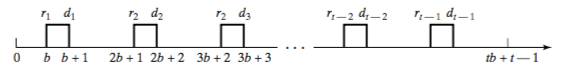
\includegraphics[width = 15cm]{Lmax1.png} \\
    図 $B.1$ : 各 $i \in \{1,\ldots,t - 1\}$ におけるジョブ $J_i$ のス
    ケジュール
  \end{center}
  各 $i \in \{1,\ldots,t - 1\}$ におけるジョブ $J_i$ を機械に割り当て
  たことで,区間 $[0,tb + t - 1]$ は長さ $b$ の $t$ 個の区間に分割され
  た.ここで,上記の条件を満たす $\mathcal{A} \subseteq 2^S$ が存在す
  ることから,$\forall A \in \mathcal{A}\big[|A| = 3 \land \sum_{a \in
    A}a = b \big]$ である.これより,各 $i' \in \{t,\ldots,4t - 1\}$ に
  おけるジョブ $J_{i'}$ は 長さ $b$ の $t$ 個の区間のいずれかに割り当
  てられる.また,各区間に割り当てられた 3 つのジョブの処理時間の和は
  $I_{(S,b)}$ より,$b$ である.
  
  以上より,上記の条件を満たす $\mathcal{A} \subseteq 2^S$ が存在するならば,
  $I_{(S,b)}$ を入力とする最大遅れ時間最小化問題に対して $\varphi(C) =
  0$ を満たす実行可能なスケジュール $C$ が存在する.
\end{proof}

\noindent \textbf{補題 4}
上記の条件を満たす $\mathcal{A} \subseteq 2^S$ が存在しないならば,
$I_{(S,b)}$ を入力とする最大遅れ時間最小化問題に対して $\varphi(C) \le
0$ を満たす実行可能なスケジュール $C$ が存在しない.\\

\begin{proof}
  各 $i \in \{1,\ldots,t - 1\}$ におけるジョブ $J_i$ は $r_i$ と $d_i =
  r_i + p_i$ の区間で処理される.(図 $B.1$)
  各 $i \in \{1,\ldots,t - 1\}$ におけるジョブ $J_i$ を機械に割り当て
  たことで,区間 $[0,tb + t - 1]$ は長さ $b$ の $t$ 個の区間に分割され
  た.ここで,上記の条件を満たす $\mathcal{A} \subseteq 2^S$ が存在し
  ないことから,$\forall A \in \mathcal{A}\big[|A| = 3 \land \sum_{a \in
    A}a \neq b \big]$ である.これより,各 $i' \in \{t,\ldots,4t - 1\}$ に
  おけるジョブ $J_{i'}$ は 長さ $b$ の $t$ 個の区間のいずれかに割り当
  てるとき,各区間のジョブの処理時間の和は $b$ ではない.\\
  以上より,上記の条件を満たす $\mathcal{A} \subseteq 2^S$ が存在しな
  いならば,$I_{(S,b)}$ を入力とする最大遅れ時間最小化問題に対して
  $\varphi(C) = 0$ を満たす実行可能なスケジュール $C$ は存在しない.
\end{proof}

補題 3 と補題 4 より,上記の条件を満たす$\mathcal{A} \subseteq 2^S$ が存在
することと,$I_{(S,b)}$ を入力とする最大遅れ時間最小化問題に対して
$\varphi(C) \le  0$
を満たす実行可能なスケジュール $C$ が存在することは,同値で
ある.
3 -PARTITION 問題の入力 $(S,b)$ に基づく $I_{(S,b)}$ の生成に要する計算時
間は,明らかに多項式時間であり,入力 $I_{(S,b)}$ の長さは,$(S, b)$
の長さに関する多項式で表すことができる.したがって,単一
機械モデルにおいて,最大遅れ時間最小化問題は強 NP 困難である.

JITジョブ荷重和最大化問題は無関連並列機械モデルにおいて,最大遅れ時間
最小化問題は単一機械モデルにおいて,NP 困難であることが証明された.
これらの問題は,2.2 でも述べたように,最大実行開始待ち時
間最小化問題と関連している.
ただ,本研究で扱う問題とこれらの問題の差分も存在し,その差分を考慮した
証明をする必要がある.

以下では,最大実行開始待ち時間最小化問題と,JIT ジョブ荷重和最大化問題
と処理開始可能時刻付き最大遅れ時間最小化問題との関連部分と差分をまとメ
ル.

\textbf{JIT ジョブ荷重和最大化問題との関連}
$w = 0$ のとき,最大実行開始待ち時間は JIT ジョブスケジューリングに対
応する.

\textbf{JIT ジョブ荷重和最大化問題との差分}
JIT ジョブ荷重和最大化問題では,納期以前に処理を完了したジョブの荷重和
最大化であるのに対し,最大実行開始待ち時間最小化問題では,全てのジョブ
の実行開始待ち時間を $w$ 以下にする必要がある.

\textbf{処理開始可能時刻付き最大遅れ時間最小化問題との関連}
$w = 0$ のとき,最大実行開始待ち時間は JIT ジョブスケジューリングに対
応する.

\textbf{処理開始可能時刻付き最大遅れ時間最小化問題との差分}
JIT ジョブ荷重和最大化問題では,納期以前に処理を完了したジョブの荷重和
最大化であるのに対し,最大実行開始待ち時間最小化問題では,全てのジョブ
の実行開始待ち時間を $w$ 以下にする必要がある.


\chapter{最大実行開始待ち時間最小化問題の計算複雑さ}
最大実行開始待ち時間最小化問題は,どの機械モデルにおいても,計算複雑さ
が明らかでない.本研究では,無関連並列機械モデルにおける最大実行開始待
ち時間最小化問題(決定問題)が NP 完全であることを示した.
\section{NP完全性の証明}
3-SAT からの還元によって,この問題が NP  完全であることを示す.3-SAT
の定義は以下である.\\

\noindent \textbf{Instance:}

ブール型の変数集合 $X$ と,$X$ 上の 3 つのリテラル
からなる集合の集合 $H$ (各 $h \in H$ は $|h| = 3$ を満たす).\\

\noindent \textbf{Question:}

$H$ を充足する真理値割り当て $f ; X \to \{0,1\}$,
つまり,
$$\displaystyle \bigwedge_{h \in H} \bigg(\bigvee_{x \in h}f(x) \lor
\bigvee_{\bar x \in h}\lnot f(x) \bigg) = 1$$
を満たす $f$ が存在するか?\\

ブール型変数の集合 $X =\{x_1, x_2,\ldots ,x_n\}$ と, $X$ 上の 3 つのリテラルからなる集合の集合 $H =\{h_1, h_2,\ldots ,h_{\lambda}\}$ の 2 項組,$(X,H)$ を任意の 3-SAT 問題の入力とする.

各 $i \in \{1,2,\ldots, n\}$ について,$\alpha_i$ を $H$ に おいて $x_i$ が現れる回数を表す自然数とし,$\beta_i$ を $H$ において $\bar x_i$ が現れる回数を表す自然数とする.
つまり,$\alpha_i = \big|\{h \in H \mid x_i \in h\}\big|$,$\beta_i = \big|\{h \in H \mid \bar x_i \in h\}\big|$
また,$\displaystyle \sum_{i \in \{1,\ldots,n\}} \alpha_i = \mathcal{A}$, $\displaystyle \sum_{i \in \{1,\ldots,n\}} \beta_i = \mathcal{B}$  とする.

ただし,各 $i \in \{1,2,\ldots, n\}$ について,$\alpha_i$, $\beta_i$ は 3 以上とする.\\
つまり,$\forall i \in \{1,\ldots,n\}\big[\alpha_i \ge 3\big]$,
$\forall i \in \{1,\ldots,n\}\big[\beta_i \ge 3\big]$

$(X.H)$ に基づき,以下のように 最大実行開始待ち時間最小化問題の入力を設定する.
$2(\mathcal{A} + \mathcal{B}) + \lambda$ 個のジョブ $\mathcal{J}$ を
$n + \lambda$ 台の無関連機械で処理する.
\begin{itemize}
\item $\mathcal{J}^t \subset \mathcal{J}$ s.t. $|\mathcal{J}^t| =
  \mathcal{A}  + \mathcal{B}$,
\item $\mathcal{J}^f \subset \mathcal{J}$
  s.t.$|\mathcal{J}^f| = \mathcal{A}  + \mathcal{B}$,
\item $\mathcal{J}^d \subset \mathcal{J}$ s.t.$|\mathcal{J}^d| =
  \lambda$
\end{itemize}
ただし,$\mathcal{J} = \mathcal{J}^t \cup \mathcal{J}^f \cup
\mathcal{J}^d$ ,$\mathcal{J}^t \cap \mathcal{J}^f = \emptyset$,$\mathcal{J}^f \cap \mathcal{J}^d = \emptyset$,$\mathcal{J}^d \cap \mathcal{J}^t = \emptyset$

つまり,$\{\mathcal{J}^t, \mathcal{J}^f,\mathcal{J}^d\}$ は $\mathcal{J}$ の分割である.\\

\noindent \textbf{実行開始待ち時間の設定}

$$w = 2$$

まず,ジョブ $\mathcal{J}^d = \{J^d_1,\ldots,J^d_{\lambda}\}$ について,
処理開始可能時刻関数 $r$ を以下のように設定する.
$$r(\mathcal{J}^d) = 3(\mathcal{A} + \mathcal{B})$$
処理時間関数 $p$ を以下のように設定する.
$$p(\mathcal{J}^d, A(\mathcal{J}^d)) = 3$$

次に,$2(\mathcal{A} + \mathcal{B})$ 個のジョブ $\mathcal{J}^t =
\{J^t_1,\ldots,J^t_{\mathcal{A} + \mathcal{B}}\}$ と $\mathcal{J}^f =
\{J^f_1,\ldots,J^f_{\mathcal{A} + \mathcal{B}}\}$ の処理開始可能時刻関
数,処理時間関数を以下のように設定する.\\

\noindent \textbf{処理開始可能時刻関数の設定}

各機械 $i \in \{1,2,\ldots,n\}$ に対応させた各ジョブの処理時間関数を設
定する.各ジョブを添え字の昇順に基づき $2n$ 個のグループに分ける. 各 $i
\in \{1,2,\ldots,n\}$ における $i$ 番目のジョブの集合を
$\mathcal{J}^t(i)$ とし,$n + i$ 番目のジョブの集合を
$\mathcal{J}^f(i)$ とする.また,グループ $i$ の $\ell$ 番目のジョブ
を $J^t(i,\ell)$ または $J^t(i,\ell)$ と表記する.
\begin{itemize}
\item ジョブの集合 $\mathcal{J}^t$ について, 各グループ $i \in
  \{1,2,\ldots, n\}$ の $\ell$ 番目のジョブの処理開始可能時刻関数を各
  $i$ における$\ell \in \{1,2,\ldots, \alpha_i + \beta_i\}$ について,
  以下のように設定する.
  $$r(J^t(i,\ell)) =
  \left\{ \begin{array}{lll} 3 \displaystyle
  \sum_{j \in \{1,\ldots,i - 1\}}(\alpha_j + \beta_j) + \ell - 1 &
  \text{if } \ell < \beta_i + 1, \\ 3 \displaystyle \sum_{j \in \{1,\ldots,i - 1\}}(\alpha_j + \beta_j) + \alpha_i + \ell - 2 & \text{otherwise} \end{array} \right.$$
                 
\item ジョブの集合 $\mathcal{J}^f$ について,各グループ $i \in \{1,2,\ldots, n\}$ の $\ell$ 番目のジョブの処理開始可能時刻を各 $i$ における $\ell \in \{1,2,\ldots,\alpha_i + \beta_i\}$ について,以下のように設定する.
  $$r(J^f(i,\ell)) =
  \left\{ \begin{array}{lll} 3 \displaystyle \sum_{j \in \{1,\ldots,i
            - 1\}}(\alpha_j + \beta_j) + \ell - 1 & \text{if } \ell = 1,
  \\ 3\displaystyle \sum_{j \in \{1,\ldots,i - 1\}}(\alpha_j + \beta_j) + \alpha_i + \ell  &
  \text{else if } \ell < \alpha_i + 1 , \\ 3\displaystyle \sum_{j \in \{1,\ldots,i - 1\}}(\alpha_j + \beta_j) + (\alpha_i + \beta_i + 4) + \ell & \text{otherwise} \end{array} \right.$$
\end{itemize}

\noindent \textbf{処理時間関数の設定}

各ジョブを処理開始可能時刻の昇順に基づき $2n$ 個のグループに分ける
\begin{itemize}
  \item グループ $i \in \{1,2,\ldots,n\}$ に機械 $i$ に対応させ,グループ
  $n + i$ にも同様に機械 $i$ を対応させる.各 $i \in \{1,2,\ldots,
  n\}$,$\ell \in \{1,2,\ldots, \alpha_i + \beta_i\}$ について,以下の
  ように設定する.
\end{itemize}
    {\footnotesize
    $$p(J^t(i,\ell), A(\mathcal{J}^t)) =
    \left\{ \begin{array}{lllll} 1 & \text{if } \ell < \beta_i \text{
                                     and } A(\mathcal{J}^t) = i, \\
              \alpha_i + 4 & \text{if } \ell = \beta_i \text{ and }
                             A(\mathcal{J}^t) = i, \\ 1 & \text{if }
                                                          \ell <
                                                          \alpha_i +
                                                          \beta_i
                                                          \text{ and }
                                                          A(\mathcal{J}^t)
                                                          = i, \\
              3(\mathcal{A} + \mathcal{B}) - \big\{ 3\displaystyle \sum_{j \in
              \{1,\ldots,i - 1\}}(\alpha_j + \beta_j) + (2\alpha_i +
              \beta_i - 2)\big \} + 3 & \text{if } \ell = \alpha_i +
                                        \beta_i \text{ and }
                                        A(\mathcal{J}^t) = i, \\
              3(\mathcal{A} + \mathcal{B}) + 3 &
                                                 \text{otherwise} \end{array} \right.$$
                                           }
{\footnotesize	
    $$p(J^f(i,\ell),A(\mathcal{J}^f)) = \left\{ \begin{array}{lllll}
                                                 \beta_i + 2 &
                                                               \text{if
                                                               } \ell
                                                               = 1
                                                               \text{
                                                               and }
                                                               A(\mathcal{J}^f)
                                                               = i, \\
                                                  1 & \text{if } \ell
                                                      < \alpha_i
                                                      \text{ and }
                                                      A(\mathcal{J}^f)
                                                      = i, \\ \alpha_i
                                                  + 5 & \text{if }
                                                        \ell =
                                                        \alpha_i
                                                        \text{ and }
                                                        A(\mathcal{J}^f)
                                                        = i, \\ 1 &
                                                                    \text{if } \ell < \alpha_i + \beta_i \text{ and } A(\mathcal{J}^f) = i, \\ 3(\mathcal{A} + \mathcal{B})- \big\{ 3\displaystyle \sum_{j \in \{1,\ldots,i - 1\}}(\alpha_j + \beta_j) + (2\alpha_i + 2\beta_i + 4)\big \} + 3 & \text{if } \ell = \alpha_i + \beta_i \text{ and } A(\mathcal{J}^f) = i , \\ 3(\mathcal{A} + \mathcal{B}) + 3 & \text{otherwise}\end{array} \right.$$
                                                              }
  \begin{itemize}
  \item 残りの各機械 $k \in \{n + 1, \ldots , n + \lambda\}$ について,
    各ジョブの処理時間を設定する
    各グループ $i \in \{1,2,\ldots,n\}$ について $x_i$ を対応させ,グ
    ループ $n + i$ について $\bar x_i$ を対応させる.つまり,$\forall
    i \in \{1,\ldots,n\}\big[x_i \to \mathcal{J}^t(i),\ \bar x_i \to
    \mathcal{J}^f(i) \big]$,
    $\mathcal{J}^t(i) = \big\{J^t(i,1),\ldots,J^t(i,\alpha_i +
    \beta_i)\big\}$,$\mathcal{J}^f(i) =
    \big\{J^f(i,1),\ldots,J^f(i,\alpha_i + \beta_i)\big\}$.
    各 $k \in \{n + 1, \ldots , n + \lambda\}$ について,
    $h_{k - n}$ に含まれるリテラルに対応するジョブを処理開始可能時刻の
    昇順で $\mathcal{T}(h_{k - n})$, $\mathcal{F}(h_{k - n})$ に入れる.
    $x_i \in h_{k - n}$ のとき,グループ $\mathcal{J}^t(i)$ のジョブを
    $\beta_i + 1$ 番目から順に $\mathcal{T}(k - n)$ に,
    $\mathcal{J}^f(i)$ のジョブを 1 番目から順に $\mathcal{F}(k - n)$ に加える.
    また,$\bar x_i \in h_{k - n}$ のとき,グループ $\mathcal{J}^f(i)$
    のジョブを $\alpha_i + 1$ 番目から順に $\mathcal{T}(k - n)$ に,
    $\mathcal{J}^t(i)$ のジョブを 1 番目から順に $\mathcal{F}(k - n)$ に加える.
    つまり,各 $k \in \{n + 1, \ldots,n + \lambda\}$,各 $i \in \{1,\ldots,n\}$ について,\\
    $count(x_i,h_j) = \big|\big\{x_i \in h_l \mid l \in \{1,\ldots,j -
    1\}\big\}\big|$ を用いて,
  \end{itemize}
    {\footnotesize
      $\mathcal{T}(h_{k - n}) = \bigg\{\big\{J^t(i,\beta_i + 1 +
      count(x_i,h_{k - n})) \mid x_i \in h_{k - n}\big\} \cap
      \big\{J^f(i,\alpha_i + 1 + count(\bar x_i, h_{k - n})) \mid \bar
      x_i \in h_{k - n}\big\}\bigg\}$\\
    }
    {\footnotesize
      $\mathcal{F}(h_{k - n}) = \bigg\{\big\{J^f(i,1 + count(
      x_i,h_{k - n})) \mid x_i \in h_{k - n} \big\} \cup \big\{J^t(i,1
      + count(\bar x_i,h_{k - n})) \mid \bar x_i \in h_{k - n}\big\} \bigg\}
      \cap J^d_{k - n}$\\
    }
    このとき,$i \in \{1,2,\ldots,n\}$,$k \in \{n + 1, \ldots , n +
    \lambda\}$,$\ell \in \{1,2,\ldots, \alpha_i + \beta_i\}$について,
    処理時間関数を次のように設定する.
  {\small
    $$p(J,A(J)) = \left\{ \begin{array}{lll} \min \big\{r(J') \mid J' \in \mathcal{F}(h_{k - n}) \wedge \big(r(J') > r(J) \big) \big\} - r(J) & \text{if } J \in \mathcal{T}(h_{k - n}), \\ \min \big\{r(J') \mid J' \in \mathcal{F}(h_{k - n}) \wedge \big(r(J') > r(J) \big) \big\} - r(J) + (4 - |h_j|) & \text{if } J \in \mathcal{F}(h_{k - n}), \\ 3(\mathcal{A} + \mathcal{B}) + 3 & \text{otherwise}\end{array} \right.$$
  }
  
このように設定した $(p,r,w)$ は最大実行開始待ち時間最小化問題の入力である.以降,$(X,H)$ に基いて前述のように設定した $(p,r,w)$ を区別して $I_{(X,H)}$ と表す.( $I_{(X,H)} = (p,r,w)$ )

以下, $H$ を充足する真理値割り当て $f : X \to \{0,1\}$ が存在する
ことと,$I_{(X,H)}$ を入力とする最大実行開始待ち時間最小化問題に対し
て,$\varphi(A,S) \le 2$ を満たす実行可能なスケジュール $(A,S)$ が
存在することが,同値であることを示す.\\

\noindent \textbf{補題 5}
$H$ を充足する真理値割り当て $f : X \to \{0,1\}$ が存在するならば,
$I_{(X,H)}$ を入力とする最大実行開始待ち時間最小化問題に対して
$\varphi(A, S) \le 2$ を満たす実行可能なス
ケジュール $(A, S)$ が存在する.\\ 

\begin{proof}
各 $i \in \{1,\ldots, n\}$ について,$f(x_i) = 1$ ならばグループ $n +
i$ の全てのジョブを,グループ $n + i$ に対応する機械 $i$ に割り当て,
そうでなければグループ $i$ の全てのジョブを,グループ $i$ に対応する機
械 $i$ に割り当てる.つまり,各 $i \in \{1,\ldots, n\}$ における各
$\ell \in \{1,\ldots,\alpha_i + \beta_i\}$ について,
$f(x_i) = 1$ ならば,$A_i := A_i \cup \mathcal{J}^f(i)$
$f(x_i) = 0$ ならば,$A_k := A_k \cup \mathcal{J}^t(i)$
$I_{(X,H)}$ の定義より,ここまでのスケジュールにおいて,機械
$\{1,\ldots, n\}$ に割り当てたジョブは処理開始可能時刻と納期の間で重複せず処理される.
よって,このとき,機械 $\{1,2,\ldots,n\}$ に割り当てられた
$\mathcal{A} + \mathcal{B}$ 個のジョブの実行開始遅れ時間は $0$ である.

上述の割り当てにより,各 $i \in \{1,\ldots,n\}$ について,$x_i$ または
$\bar x_i$ に対応するジョブ $\mathcal{J}^t(i)$ または
$\mathcal{J}^f(i)$ のどちらか一方が機械 $i$ に割り当てられた.このとき,
上図より,機械 $i$ におけるジョブの完了時刻は $3(\mathcal{A} +
\mathcal{B}) + 3$ であるので,いずれのジョブも機械 $i$ に割り当てることができない.
よって,残りのジョブについては,各 $k \in \{n + 1,\ldots,n +
\lambda\}$ における機械 $k$ に割り当てる.

前提条件より,$f$ が $H$ を充足することから,各 $i \in \{1,\ldots,n\}$,
$j \in \{1, \ldots, \lambda \}$ について,$f(x_i) = 1$ を満たす $x_i
\in h_j$ か,$f(x_i) = 0$ を満たす $\bar x_i \in h_j$ を満たすリテラルは必ず存在する.
ここで,与えられた $j \in \{1, \ldots, \lambda \}$ について,$f(x_i) =
1$ を満たす $x_i \in h_j$ を見つけたと仮定する.グループ $i$ のジョブ
の集合 $\mathcal{J}^t(i)$ は,$f(x_i) = 1$ であることから,
$\{1,\ldots,n\}$ のいずれの機械にも割り当てられていないので,そのよう
なグループ $i$ のジョブの集合 $\mathcal{J}^t(i)$ は必ず存在する.
同様に,$f(x_i) = 0$ を満たす $\bar x_i \in h_j$ を見つけたと仮定する.
グループ $n + i$ のジョブの集合 $\mathcal{J}^f(i)$ のうち,いずれの機
械にも割り当てられていないグループ $n + i$ を見つける.先程と同じ議論
で,そのようなグループ $n + i$ のジョブ $\mathcal{J}^f(i)$ は必ず存在する.

各 $j \in \{1, \ldots, \lambda \}$ における $h_j$ に対応するジョブの集
合 $\mathcal{T}(h_j)$ または $\mathcal{F}(h_j)$ のジョブを処理開始可能
時刻の昇順で機械 $j$ に割り当てる.
このとき,1 に割り当てられたリテラルに対応するジョブが少なくとも 1 つ
各機械に割り当てられているので,各機械におけるジョブの完了時刻は高々
$3(\mathcal{A} + \mathcal{B}) + 2$ である.
ここで,各 $j \in \{1,\ldots,\lambda\}$ における $J^d_j$ を各機械 $j$
に 1 つずつ割り当てる.
このとき,$J^d$ の処理開始可能時刻は $I_{(X,H)}$ より,$3(\mathcal{A}
+ \mathcal{B})$ であるので,実行開始待ち時間は高々 2 である.

今までの議論より,$\mathcal{A} + \mathcal{B}$ 個のジョブを機械 $i \in
\{1,\ldots,n\}$ に,$\mathcal{A} + \mathcal{B}$ 個のジョブを機械 $k \in\{n + 1, \ldots, n + \lambda\}$ に,$\lambda$ 個のジョブを機械 $k \in\{n + 1, \ldots, n + \lambda\}$ に割り当てた.
このとき,全てのジョブをいずれかの機械に割り当てており,全てのジョブに
関して,実行開始待ち時間は高々 2 であることから,$f$ が $H$ を充足す
るとき,$I_{(X,H)}$ において,$\varphi(A,S) \le 2$ を満たす.
\end{proof}
  
\noindent \textbf{補題 6}
$H$ を充足する真理値割り当て $f : X \to \{0,1\}$ が存在しないならば,
$I_{(X,H)}$ を入力とする最大実行開始待ち時間最小化問題に対して
$\varphi(A, C) \le 2$ を満たす実行可能なス
ケジュール $(A, S)$ が存在sしない.\\ 

\begin{proof}
$f$ が $H$ を充足しないことから,各 $j \in \{1, \ldots, \lambda \}$ に
ついて,$f(x_i) = 1$ を満たす $x_i \in h_j$ か,$f(x_i) = 0$ を満たす
$\bar x_i \in h_j$ が1つも存在しない機械 $j \in \{1,\ldots, \lambda\}$ が必ず存在する.
その機械を $j^{\prime}$ とし,以下,機械 $j^{\prime}$ 上のスケジュールについて述べる.
\begin{itemize}
\item $x_i \in h_j^{\prime}$ または $\bar x_i \in h_j^{\prime}$ に対応
  するジョブのみを機械 $j^{\prime}$ に割り当てた場合
  \begin{itemize}
  \item $|h_j^{\prime}| = 3$ のとき
    
    $I_{(X,H)}$ より,それらのジョブは,スケジュールにおける次のジョブ
    の処理開始可能時刻を 1 超える処理時間を持つ.$h_{j^{\prime}}$ に含
    まれる $x_i$ 以外の残りの 2 つのリテラルに対応するジョブについても
    同様に機械 $j^{\prime}$ に割り当てる.
    $I_{(X,H)}$ より,機械 $j^{\prime}$ におけるジョブの完了時刻は
    $3(\mathcal{A} + \mathcal{B}) + 3$ となる.ここで,$j \in
    \{1,\ldots,\lambda\}$ におけるジョブ $J^d_{j^{\prime}}$ をそれらの
    ジョブの後に割り当てるとき,ジョブ $J^d_{j^{\prime}}$ に 3 の実行開始待ち時間が発生する.
  \item $|h_j^{\prime}| = 2$ のとき,
    
    $|h_j^{\prime}| = 3$ のときと同様に割り当てる.$I_{(X,H)}$ より,
    各ジョブはスケジュールにおける次のジョブの処理開始可能時刻を 2 超
    える処理時間を持つ.$h_{j^{\prime}}$ に含まれる $x_i$ 以外の残りの
    1 つのリテラルに対応するジョブについても同様に機械 $j^{\prime}$ に割り当てる.
    $I_{(X,H)}$ より,機械 $j^{\prime}$ におけるジョブの完了時刻は
    $3(\mathcal{A} + \mathcal{B}) + 4$ となる.ここで,$j \in
    \{1,\ldots,\lambda\}$ において,機械に割り当てられていないジョブ
    $J^d_{j^{\prime}}$ をそれらのジョブの後に割り当てるとき,ジョブ
    $J^d_{j^{\prime}}$ に 4 の実行開始待ち時間が発生する.
  \item  $|h_j^{\prime}| = 1$ のとき,
    
    $|h_j^{\prime}| = 3$ のときと同様に割り当てる.$I_{(X,H)}$ より,
    各ジョブはスケジュールにおける次のジョブの処理開始可能時刻を 3 超える処理時間を持つ.
    $I_{(X,H)}$ より,機械 $j^{\prime}$ におけるジョブの完了時刻は
    $3(\mathcal{A} + \mathcal{B}) + 3$ となる.ここで,$j \in
    \{1,\ldots,\lambda\}$ において,機械に割り当てられていないジョブ
    $J^d_{j^{\prime}}$ をそれらのジョブの後に割り当てるとき,ジョブ
    $J^d_{j^{\prime}}$ に 3 の実行開始待ち時間が発生する.
  \end{itemize}
\item $x_k \notin h_j$ または $\bar x_k \notin h_j$ に対応するジョブを
  割り当てた場合
  
  機械 $j^{\prime}$ にそのようなジョブを1 つでも割り当てた場合,
  $I_{(X,H)}$ より,機械 $j^{\prime}$ におけるジョブの完了時刻は
  $3(\mathcal{A} + \mathcal{B}) + 3$ となる.ここで,$j \in
  \{1,\ldots,\lambda\}$ において,機械に割り当てられていないジョブ
  $J^d_{j^{\prime}}$ をそれらのジョブの後に割り当てるとき,ジョブ
  $J^d_{j^{\prime}}$ に 3 の実行開始待ち時間が発生する.
\item 上記の 2 つのケースにおいて,$j \in \{1,\ldots,\lambda\}$ におい
  て,機械に割り当てられていないジョブ $J^d_{j^{\prime}}$ を機械 $i
  \in \{1,\ldots,n\}$ に割り当てた場合 $I_{(X,H)}$ より,ジョブ
  $J^d_{j^{\prime}}$ に 3 の実行開始待ち時間が発生する.
\end{itemize}
以上より,各 $j \in \{1,\ldots,\lambda\}$ における機械 $j$ にどのジョ
ブをどのように割り当てたしたとしても,少なくとも 1 つ実行開始待ち時間が3以上になる機械が存在する.
よって,$H$ を充足する真理値割り当て $f$ が存在しないとき,実行開始待
ち時間が 2 以下となるスケジュールは存在しない.
\end{proof}

補題 5 と補題 6 より,$H$ を充足する真理値割り当て $f : X \to \{0,
1\}$ が存在することと,$I_{(X,H)}$ を入力とする最大実行開始待ち時間
最小化問題に対して $\varphi(A, S) \le 2$
を満たす実行可能なスケジュール $(A, S)$ が存在することは,同値で
ある.
3 -SAT 問題の入力 $(X,H)$ に基づく $I_{(X,H)}$ の生成に要する計算時
間は,明らかに多項式時間であり,入力 $I_{(X,H)}$ の長さは,$(X, H)$
の長さに関する多項式で表すことができる.したがって,無関連並列
機械モデルにおいて機械数が入力の一部の場合, 最大実行開始待ち時間
最小化問題は NP 完全である.

\section{機械モデルの違いが問題の計算複雑さに与える影響}

\chapter{計算論的分析}
\section{実行可能なスケジュール}
\section{解法と評価方法}
\section{開発した解法の評価}

\chapter{結論}
\section{研究成果}
\section{今後の課題}

\bibliographystyle{splncs03}
\bibliography{thesis}

\chapter*{謝辞}

\begin{flushright}
  2017年1月31日 \氏名
\end{flushright}
\endmatter 
\end{document}
